\section{Testing Phases}

\subsection{Unit Testing}
Unit testing was done at very point essentially, as we were in the coding phase. Every building block was tested rigorously using multiple cases. We tested for recognition of dataypes, variables , expression statements and functions initially, and then moved on to AST generation.

\subsection{Integration Testing}
In this phase,the various modules were put together and tested incrementally again. So once the AST could be generated, we moved on to test the semantic analysis and code generation.

\subsection{System Testing}
System testing entailed end to end testing of our entire language framework. The input program written in QLang is fed to the compiler and it gives out the final output of the program, having passed through the parsing, scanning, compiling, code generation and execution phases. The final results were piped to an output file where we could see all the outputs.


\section{Automation and Implementation}
A shell script was written in order to automate the test cases at each level, syntax, semantic, code
generation and accurate execution. 
Our file is called runTests.sh, located in the 'test' folder. It takes a folder having QLang program files, and the operation to be done on them as arguments. The outputs of the respective operation can be seen in the corresponding output file. 


The operation options available are :

a : Parsing, scanning and AST generation. \\
s : SAST generation.\\
g : Code generation.\\
c : Generated code is compiled.\\
e : Generated executable is run, to generate the program's outputs.\\ 

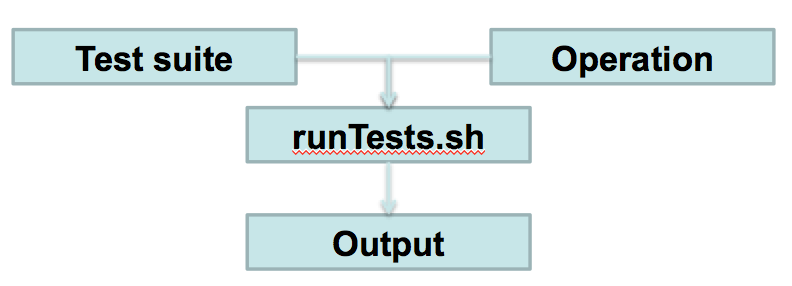
\includegraphics[scale=0.60]{Test_diagrams/2.png}

The operations mentioned above are each inclusive of the operations mentioned above them. That means, if you enter the 'g' option, runTests.sh will perform the tasks under 'a','s' and then the operations specific to 'g' as well.

The second argument is the folder that has the input program files. We have acronyms for two folder that are standard to our implementation, the SemanticSuccess and the SemanticFailures. So to run the sast generation on the files in SemanticSuccess folder, we would write :
\\
\begin{lstlisting}
sh runTests.sh s ss.
\end{lstlisting}

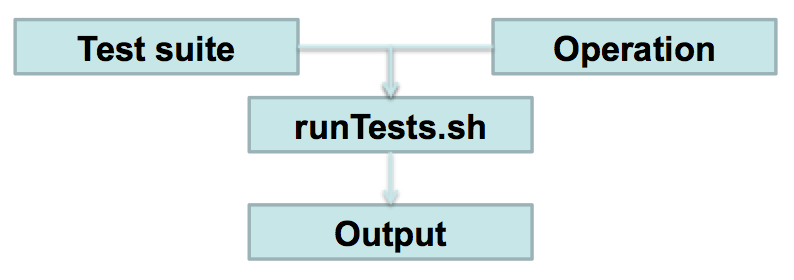
\includegraphics[scale=0.60]{Test_diagrams/1.png}


The entire code of this script can be seen in the appendix.


\section{Sample test programs}

The effort has been to exhaustively test every kind of execution scenario, in what can be a typical user program. We have created many test files to showcase varied kinds of programs that can be written in QLang, as can be seen in the contents of the SemanticSuccess and SemanticFailures folders.

The rationale is to make sure that syntactically or semantically incorrect programs are not compiled and echo corresponding meaningful error messages to the user, and that correct programs are accepted and executed correctly.

Hence, we have separate test programs to test all kinds of unary and binary operations on all datatypes that our language supports, and also for all kinds of statements and possible combinations of expressions. 
Though the test suite is too large to be included in this section, here are a few sample success and failure cases that showcase different applications of our language :


For instance, break\_continue.ql is a QLang program as follows :

\begin{lstlisting}

def func_test(int a) : int ret_name { 
        
        int i;

        for(i from 0 to 2 by 1)
        a=a+5;

        for(i from 2 to 0 by -1)
        {
            a=a*10;
            print(a);
            break;
        }

        for(i from 1 to 5)
        {
            print(a);
            continue;
            a=a*10;

        }

    ret_name = a;
}

def compute(): int trial {

   trial = func_test(20);
} 
\end{lstlisting}

It generates break\_continue.cpp as below upon passing it through the code generation code
\begin{lstlisting}

#include <iostream>
#include <complex>
#include <cmath>
#include <Eigen/Dense>
#include <qlang>
using namespace Eigen;
using namespace std;
        
int func_test (int a )
{
	int i;
	int ret_name;
 

    for (int i = 0; i < 2; i = i + 1){
        	a = a + 5;

        }
    for (int i = 2; i < 0; i = i +   -1){
        
	{
	a = a * 10;

	cout << a << endl;

break;
	}

        }
    for (int i = 1; i < 5; i = i + 1){
        
	{
	cout << a << endl;

continue;
	a = a * 10;

	}

        }	ret_name = a;

	return ret_name;
}
int main ()
{
	int trial;
 
	trial = func_test(20);

	std::cout << trial << endl;

	return 0;
}
\end{lstlisting}


and the generated output of this is :

\begin{lstlisting}
30
30
30
30
30
\end{lstlisting}


Another example we consider is  mat\_qubit.ql


\begin{lstlisting}
def func_test(mat a, mat b) : mat ret_name { 
        
        ret_name = a*b;

}


def compute(int a):mat trial {
	
	 mat zero;
	 mat one;

	 zero = |0>;
	 one  = |1>;

     trial = func_test(H,zero);
     printq(trial);

     trial = func_test(H,one);
     printq(trial);

}
\end{lstlisting}

It generates mat\_qubit.cpp as below :


\begin{lstlisting}
#include <iostream>
#include <complex>
#include <cmath>
#include <Eigen/Dense>
#include <qlang>
using namespace Eigen;
using namespace std;
        
MatrixXcf func_test (MatrixXcf a,MatrixXcf b )
{
	MatrixXcf ret_name;
 
	ret_name = a * b;

	return ret_name;
}
int main ()
{
	MatrixXcf zero;
	MatrixXcf one;
	MatrixXcf trial;
 
	zero = genQubit("0",0);
	one = genQubit("1",0);
	trial = func_test(H,zero);
	cout << vectorToBraket(trial) << endl;
	trial = func_test(H,one);
	cout << vectorToBraket(trial) << endl;

	std::cout << trial << endl;

	return 0;
}
\end{lstlisting}

and it generates the qubits in the output as well, like :

\begin{lstlisting}
(0.707107)|0> + (0.707107)|1>
(0.707107)|0> + (-0.707107)|1>
(0.707107,0)
(-0.707107,0)
\end{lstlisting}

One more program we can show here is a demonstration of the capacity of QLang to emulate Quantum algorithms. The following program runs the Deutsch-Jozsa algorithm.


\begin{lstlisting}
def measure (mat top) : mat outcome{
        
        mat ad;

        ad = adj(top);
        outcome = top * ad;
}

def hadamard (int n) : mat gate{
        
        int i;
        gate = H;

        for (i from 0 to n-1 by 1){
            gate = gate @ H; 
        }
}

def topqubit (int n) : mat input{

        int i;
        input = |0>;

        for (i from 0 to n-1 by 1){
                input = input @ |0>;
        }          
}

def deutsch (int n, mat U) : float outcomeZero{

        mat bottom; mat top; mat input;
        mat hadtop; mat meas;

        bottom = |1>;
        top = topqubit(n);
        input = top @ bottom;
        
        hadtop = hadamard(n);
        input = (hadtop @ H)*input;
        input = U * input;
        input = (hadtop @ IDT)*input;
        meas = measure(top);

        input = (meas @ IDT)* input;
        outcomeZero = norm(input);
}


def compute () : float outcome{

        int n; mat Ub; mat Uc;

        n = 1;
        Ub = [(1,0,0,0)(0,1,0,0)(0,0,0,1)(0,0,1,0)];
        Uc = [(1,0,0,0)(0,1,0,0)(0,0,1,0)(0,0,0,1)];

        outcome = deutsch(n, Ub);
        print(outcome);
        
        outcome = deutsch(n, Uc);
        print(outcome);

        n = 2;
        Ub = [(1,0,0,0,0,0,0,0) 
              (0,1,0,0,0,0,0,0)
              (0,0,1,0,0,0,0,0)
              (0,0,0,1,0,0,0,0) 
              (0,0,0,0,0,1,0,0) 
              (0,0,0,0,1,0,0,0)
              (0,0,0,0,0,0,0,1)
              (0,0,0,0,0,0,1,0)];

        outcome = deutsch(n, Ub);
}
\end{lstlisting}

It creates the C++ code as follows :

\begin{lstlisting}

#include <iostream>
#include <complex>
#include <cmath>
#include <Eigen/Dense>
#include <qlang>
using namespace Eigen;
using namespace std;
        
MatrixXcf measure (MatrixXcf top )
{
	MatrixXcf ad;
	MatrixXcf outcome;
 
	ad =   top.adjoint();
	outcome = top * ad;

	return outcome;
}
MatrixXcf hadamard (int n )
{
	int i;
	MatrixXcf gate;
 
	gate = H;

    for (int i = 0; i < n - 1; i = i + 1){
        
	{
	gate = tensor(gate, H);

	}

        }
	return gate;
}
MatrixXcf topqubit (int n )
{
	int i;
	MatrixXcf input;
 
	input = genQubit("0",0);

    for (int i = 0; i < n - 1; i = i + 1){
        
	{
	input = tensor(input, genQubit("0",0));

	}

        }
	return input;
}
float deutsch (int n,MatrixXcf U )
{
	MatrixXcf bottom;
	MatrixXcf top;
	MatrixXcf input;
	MatrixXcf hadtop;
	MatrixXcf meas;
	float outcomeZero;
 
	bottom = genQubit("1",0);
	top = topqubit(n);
	input = tensor(top, bottom);
	hadtop = hadamard(n);
	input = tensor(hadtop, H) * input;
	input = U * input;
	input = tensor(hadtop, IDT) * input;
	meas = measure(top);
	input = tensor(meas, IDT) * input;
	outcomeZero =   input.norm();

	return outcomeZero;
}
int main ()
{
	int n;
	MatrixXcf Ub;
	MatrixXcf Uc;
	float outcome;
 
	n = 1;
	Ub = (Matrix<complex<float>, Dynamic, Dynamic>(4,4)<<1,0,0,0,0,1,0,0,0,0,0,1,0,0,1,0).finished();
	Uc = (Matrix<complex<float>, Dynamic, Dynamic>(4,4)<<1,0,0,0,0,1,0,0,0,0,1,0,0,0,0,1).finished();
	outcome = deutsch(n,Ub);
	cout << outcome << endl << endl;
	outcome = deutsch(n,Uc);
	cout << outcome << endl << endl;
	n = 2;
	Ub = (Matrix<complex<float>, Dynamic, Dynamic> (8,8)       <<1,0,0,0,0,0,0,0,0,1,0,0,0,0,0,0,0,0,1,0,0,0,0,0,0,0,0,1,0,0,0,0,0,0,0,0,0,1,0,0,0,0,0,0,1,0,0,0,0,0,0,0,0,0,0,1,0,0,0,0,0,0,1,0)
	.finished();
	outcome = deutsch(n,Ub);

	std::cout << outcome << endl;

	return 0;
}
\end{lstlisting}

The output of this exceution is :

\begin{lstlisting}
0

1

0
\end{lstlisting}



Following programs show the ability of the semantic analyzer to catch incorrect programs. For instance, the program:

\begin{lstlisting}
def func_test1(int z) : int ret_name { 
        int a;
        int b;
        int d;
        a = z;
        ret_name = z;

}
def func_test1(int z) : int ret_name2 { 

        ret_name2 = z;

}
def compute( int a):int trial {
      
      trial = func_test1(4);
}

\end{lstlisting}


gives the error :
\begin{lstlisting}
Fatal error: exception Analyzer.Except("Invalid function declaration: func_test1 was already declared")
\end{lstlisting}


whereas the sample program

\begin{lstlisting}
def func_test(float z) : float ret_name { 
        
        float a; 
        a = 5.8;
       
        ret_name = z;  
}
\end{lstlisting}


would give the error :
\begin{lstlisting}
Fatal error: exception Analyzer.Except("Missing 'compute' function")
\end{lstlisting}

More such pass and fail test cases can be found in the appendix and in our project folder.





